%%
%% This is file `sample-authordraft.tex',
%% generated with the docstrip utility.
%%
%% The original source files were:
%%
%% samples.dtx (with options: `authordraft')
%% 
%% IMPORTANT NOTICE:
%% 
%% For the copyright see the source file.
%% 
%% Any modified versions of this file must be renamed
%% with new filenames distinct from sample-authordraft.tex.
%% 
%% For distribution of the original source see the terms
%% for copying and modification in the file samples.dtx.
%% 
%% This generated file may be distributed as long as the
%% original source files, as listed above, are part of the
%% same distribution.  (The sources need not necessarily be
%% in the same archive or directory.)
%%
%% Commands for TeXCount
%TC:macro \cite [option:text,text]
%TC:macro \citep [option:text,text]
%TC:macro \citet [option:text,text]
%TC:envir table 0 1
%TC:envir table* 0 1
%TC:envir tabular [ignore] word
%TC:envir displaymath 0 word
%TC:envir math 0 word
%TC:envir comment 0 0
%%
%%
%% The first command in your LaTeX source must be the \documentclass command.
\documentclass[sigconf,authordraft]{acmart}
%% NOTE that a single column version may required for 
%% submission and peer review.  This can be done by changing
%% the \doucmentclass[...]{acmart} in this template to 
%% \documentclass[manuscript,screen]{acmart}
%% 
%% To ensure 100% compatibility, please check the white list of
%% approved LaTeX packages to be used with the Master Article Template at
%% https://www.acm.org/publications/taps/whitelist-of-latex-packages 
%% before creating your document.  The white list page provides 
%% information on how to submit additional LaTeX packages for 
%% review and adoption.
%% Fonts used in the template cannot be substituted; margin 
%% adjustments are not allowed.

%%
%% \BibTeX command to typeset BibTeX logo in the docs
\AtBeginDocument{%
 \providecommand\BibTeX{{%
 \normalfont B\kern-0.5em{\scshape i\kern-0.25em b}\kern-0.8em\TeX}}}

%% Rights management information.  This information is sent to you
%% when you complete the rights form.  These commands have SAMPLE
%% values in them; it is your responsibility as an author to replace
%% the commands and values with those provided to you when you
%% complete the rights form.
\setcopyright{acmcopyright}
\copyrightyear{2018}
\acmYear{2018}
\acmDOI{XXXXXXX.XXXXXXX}

%% These commands are for a PROCEEDINGS abstract or paper.
\acmConference[Conference acronym 'XX]{Make sure to enter the correct
 conference title from your rights confirmation emai}{June 03--05,
 2018}{Woodstock, NY}
%
% Uncomment \acmBooktitle if th title of the proceedings is different
% from ``Proceedings of ...''!
%
%\acmBooktitle{Woodstock '18: ACM Symposium on Neural Gaze Detection,
% June 03--05, 2018, Woodstock, NY} 
\acmPrice{15.00}
\acmISBN{978-1-4503-XXXX-X/18/06}


%%
%% Submission ID.
%% Use this when submitting an article to a sponsored event.  You'll
%% receive a unique submission ID from the organizers
%% of the event, and this ID should be used as the parameter to this command.
%%\acmSubmissionID{123-A56-BU3}

%%
%% The majority of ACM publications use numbered citations and
%% references.  The command \citestyle{authoryear} switches to the
%% "author year" style.
%%
%% If you are preparing content for an event
%% sponsored by ACM SIGGRAPH, you must use the "author year" style of
%% citations and references.
%% Uncommenting
%% the next command will enable that style.
%%\citestyle{acmauthoryear}

%%
%% end of the preamble, start of the body of the document source.
\begin{document}

%%
%% The "title" command has an optional parameter,
%% allowing the author to define a "short title" to be used in page headers.
\title{Leap Motion Virtual Piano}

%%
%% The "author" command and its associated commands are used to define
%% the authors and their affiliations.
%% Of note is the shared affiliation of the first two authors, and the
%% "authornote" and "authornotemark" commands
%% used to denote shared contribution to the research.

\author{Maggie Funston}
\affiliation{%
 \institution{Colorado State University}
 \city{Fort Collins}
 \state{Colorado}
 \country{United States}}
\email{mfunston@rams.colostate.edu}




%%
%% By default, the full list of authors will be used in the page
%% headers.  Often, this list is too long, and will overlap
%% other information printed in the page headers.  This command allows
%% the author to define a more concise list
%% of authors' names for this purpose.
\renewcommand{\shortauthors}{Trovato and Tobin, et al.}

%%
%% The abstract is a short summary of the work to be presented in the
%% article.
\begin{abstract}
 Virtual Instruments using gesture based technology are becoming increasingly popular.  This paper aims to explore the possibility of replacing physical pianos with motion sensor virtual ones in K-12 schools because of extensive budget cuts.
 A leap motion device and unity were used to create this virtual motion sensor piano.
\end{abstract}

%%
%% The code below is generated by the tool at http://dl.acm.org/ccs.cfm.
%% Please copy and paste the code instead of the example below.
%%
% \begin{CCSXML}
% <ccs2012>
% <concept>
% <concept_id>10010520.10010553.10010562</concept_id>
% <concept_desc>Computer systems organization~Embedded systems</concept_desc>
% <concept_significance>500</concept_significance>
% </concept>
% <concept>
% <concept_id>10010520.10010575.10010755</concept_id>
% <concept_desc>Computer systems organization~Redundancy</concept_desc>
% <concept_significance>300</concept_significance>
% </concept>
% <concept>
% <concept_id>10010520.10010553.10010554</concept_id>
% <concept_desc>Computer systems organization~Robotics</concept_desc>
% <concept_significance>100</concept_significance>
% </concept>
% <concept>
% <concept_id>10003033.10003083.10003095</concept_id>
% <concept_desc>Networks~Network reliability</concept_desc>
% <concept_significance>100</concept_significance>
% </concept>
% </ccs2012>
% \end{CCSXML}

\ccsdesc[500]{Human Computer Interaction~User Studies}
\ccsdesc[300]{Human Computer Interaction~Gestural Input}

%%
%% Keywords.  The author(s) should pick words that accurately describe
%% the work being presented.  Separate the keywords with commas.
\keywords{Leap Motion, Virtual Piano, Virtual Instruments, School, Music Programs, School Districts, Budget Cuts, Unity}

%%
%% This command processes the author and affiliation and title
%% information and builds the first part of the formatted document.
\maketitle

\section{Introduction}

Music has existed for a very long time.  Humans started creating musical instruments at least 40,000 years ago \cite{Smithsonian}.  With the advancement of technology, we have been able to change not only the way we access music, but the way we listen to it as well.  Advances in technology have also allowed us to change the way we play music.  The early 1990’s marks the start of virtual reality musical instruments \cite{swed_1994}.  While virtual reality has existed for a long time, it wasn’t until recently that virtual reality has exploded and become significantly more advanced.  Gesture recognition technology, often used alongside VR, is becoming more advanced as well.  Because these technologies are becoming so advanced, they are aiding in the accessibility and popularity of virtual reality instruments.

Using UltraLeap's Leap Motion Controller, I built a virtual motion sensor piano.  The Leap Motion Controller is a hand tracking device.  When plugged into a computer, users can hold their hands above the device and it senses the motions the users make.  These motions are reflected on the computer screen as a set of hands, allowing the user to interact and play with the virtual piano.

Building virtual instruments using the Leap Motion Controller has the potential to help school districts give their students access to the music programs that have been cut across the country.  This project will look into replacing physical instruments with virtual reality and motion gesture instruments, specifically the piano.  This project will build on previous projects and research regarding virtual instruments to determine if a virtual motion sensor piano can be a suitable replacement for a physical piano.

Since 2008, school districts across the country have gone through significant budget cuts \cite{mcdonald_2016}.  Both art and music programs have faced the bulk of these budget cuts, as they are often considered to be extracurricular and not as important as some of the other subjects such as mathematics or science.  When students are able to partake in their school’s music program, they are not only more likely to graduate and go to college, but also suffer less from anxiety, depression, and stress \cite{vinnard22, mcdonald_2016}.  Students are likely to face repercussions and could have difficulties in their life because their schools chose not to fund their music and art programs.  One study performed in 2019, along with past studies, found that school-based music programs have a positive effect on childrens’ literacy-related language skills and memory functions \cite{Lukas}.  Another study performed in 2021 looked at children between the ages of 4 and 5, and their socio-emotional development in relation to music programs.  This study found that the younger children had an increase in social interaction and independence skills while the older children had an increase in their comprehension of emotions, but a decrease in cooperation skills \cite{Boucher}.

It makes sense music programs are cut only because they are expensive.  Musical instruments can cost school districts a fortune.  School districts need to make sure there is enough instruments for all participating students.  Depending on the instrument, it can cost a school between \$200 - \$3000.  Even if the school receives a discount, this is still a lot of money.  Then there is also the cost of maintenance for these instruments.  The technology used to create virtual instruments can be expensive, it is still cheaper physical instruments and the schools most likely already purchase some of the things necessary like a computer.  Using this technology would also allow for the switching between multiple musical instruments.  There would not be the need to make sure there are enough instruments then, just enough technology.  For example, the leap motion device could be used as a piano, but it could probably be used as a xylophone as well.  This would allow for significant savings since pianos and xylophones costs at least \$1000 each while the leap motion device ranges between \$100 and \$150.


\section{Background}
In recent years, gesture based technology has advanced rapidly which has led to more people using various forms of gesture based technology in their every day lives.  For example, some doctors use gesture based technology while performing surgery, while some people play video games using the the Nintendo Wii, or the Xbox Kinnect, both involving gesture based technology.  There have also been numerous studies done in relation to gesture based technology with virtual instruments, specifically using the Leap Motion device.  There is a very wide range of possibilities for this technology.

Gesture based technology can be used in Augmented Reality (AR).  A leap motion device can be used to track hand positions and gestures in Marker-less AR.  Marker-less AR frameworks involve overlaying 3D virtual objects in the user's real environment with a camera and screen.  In 2016, a leap motion device was used to create a Marker-less AR framework which allowed for interaction with the augmented objects.  Different gestures would allow for users to shoot a fireball out of their hand or even interact with bubbles.  This setup allowed for a cheaper solution for Augmented Reality \cite{Zhao}.

As gesture based technology has advanced, it has allowed for the development and creation of more advanced virtual musical instruments.  Ridho Rahman Hariadi and Imam Kuswardayan, both lecturers at a university in Indoneisa looked at playing various traditional Indonesian musical instruments using a Leap Motion device \cite{Hariadi}.  They used a laptop for visualization and the leap motion device was used to sense and gestures provided by the user.  The two lecturers had users choose one of the five instruments to play.  They had the users go through five different testing scenarios, and measured user experience and application interface via a survey provided to the users.  Hariadi and Kuswardayan concluded that Virtual Indonesian Musical Instruments can be used as an alternative way to learning traditional Indonesian musical instruments.

Gesture based technology has also been used to teach elementary students about music performance.  Ikhsan Perdana created 2 software programs using the leap motion device to teach these students.  The first program was relatively simple, and would allow students to play a melody, using one hand to control the pitch and another hand to determine if the sound was playing.  The second software a game for the students to show what they learned and remembered from the first software.  This game was set up similar to Rock Band and Guitar hero \cite{Perdana}.  

Kate Sanborn created a virtual flute and tutoring system to not only help students learn how to play flute, but also broaden music accessibility as not everyone can afford a physical instrument.  Sanborn created the AirFlute using leap motion device and web interface.  The leap motion device was used to track the students hand movement so that when they pressed a key on the flute, the corresponding sound is played \cite{Sanborn}.

Gesture based technology isn't the only way to create virtual instruments.  Sometimes, multi-touch interfaces will be necessary.  In 2012, a group of people from the University of North Carolina created a multi-touch table top percussion instrument.  Groups of users were able to play various instruments together on the same table top.  It was determined that participant's of all experience levels found the system easy intuitive and easy to use \cite{Ren}.

Alexi Sourin used gesture technology to create a virtual theremin.  The theremin is the first electronic instrument, and is played without physical contact.  The leap motion device was used to sense a user's hand motion, however on the screen instead of displaying the instrument and a user's hands, a piano that was displayed.  There would be a cursor over the key that represented the note the user was playing \cite{Sourin}.

Gesture based technology has been used in numerous cases to successfully create virtual, motion sensor musical instruments.

\section{Methods}
\subsection{Participants}
This study will use a sample size of 10 participants, ranging in ages 20 to 53.  Participants can have any range of experience in playing a piano.

\subsection{Materials/Apparatus}
The materials used in this study are a Leap Motion Device, a computer, and a physical piano.  The Leap Motion Device was used to capture all hand gestures from the participants playing the virtual piano.  The computer was used to run the Unity program, and display the virtual piano for users to see.  The real piano was used so participants could play the real piano, and then the virtual piano and compare their experiences.  

% EXPAND UPON THIS
The creation of the virtual piano involved adapting a past virtual piano project in Unity.  The virtual piano object was designed in blender by the team who initially created this project.  All the functionality was done through Unity and the Leap Motion software.

\begin{figure}[h]
\centering
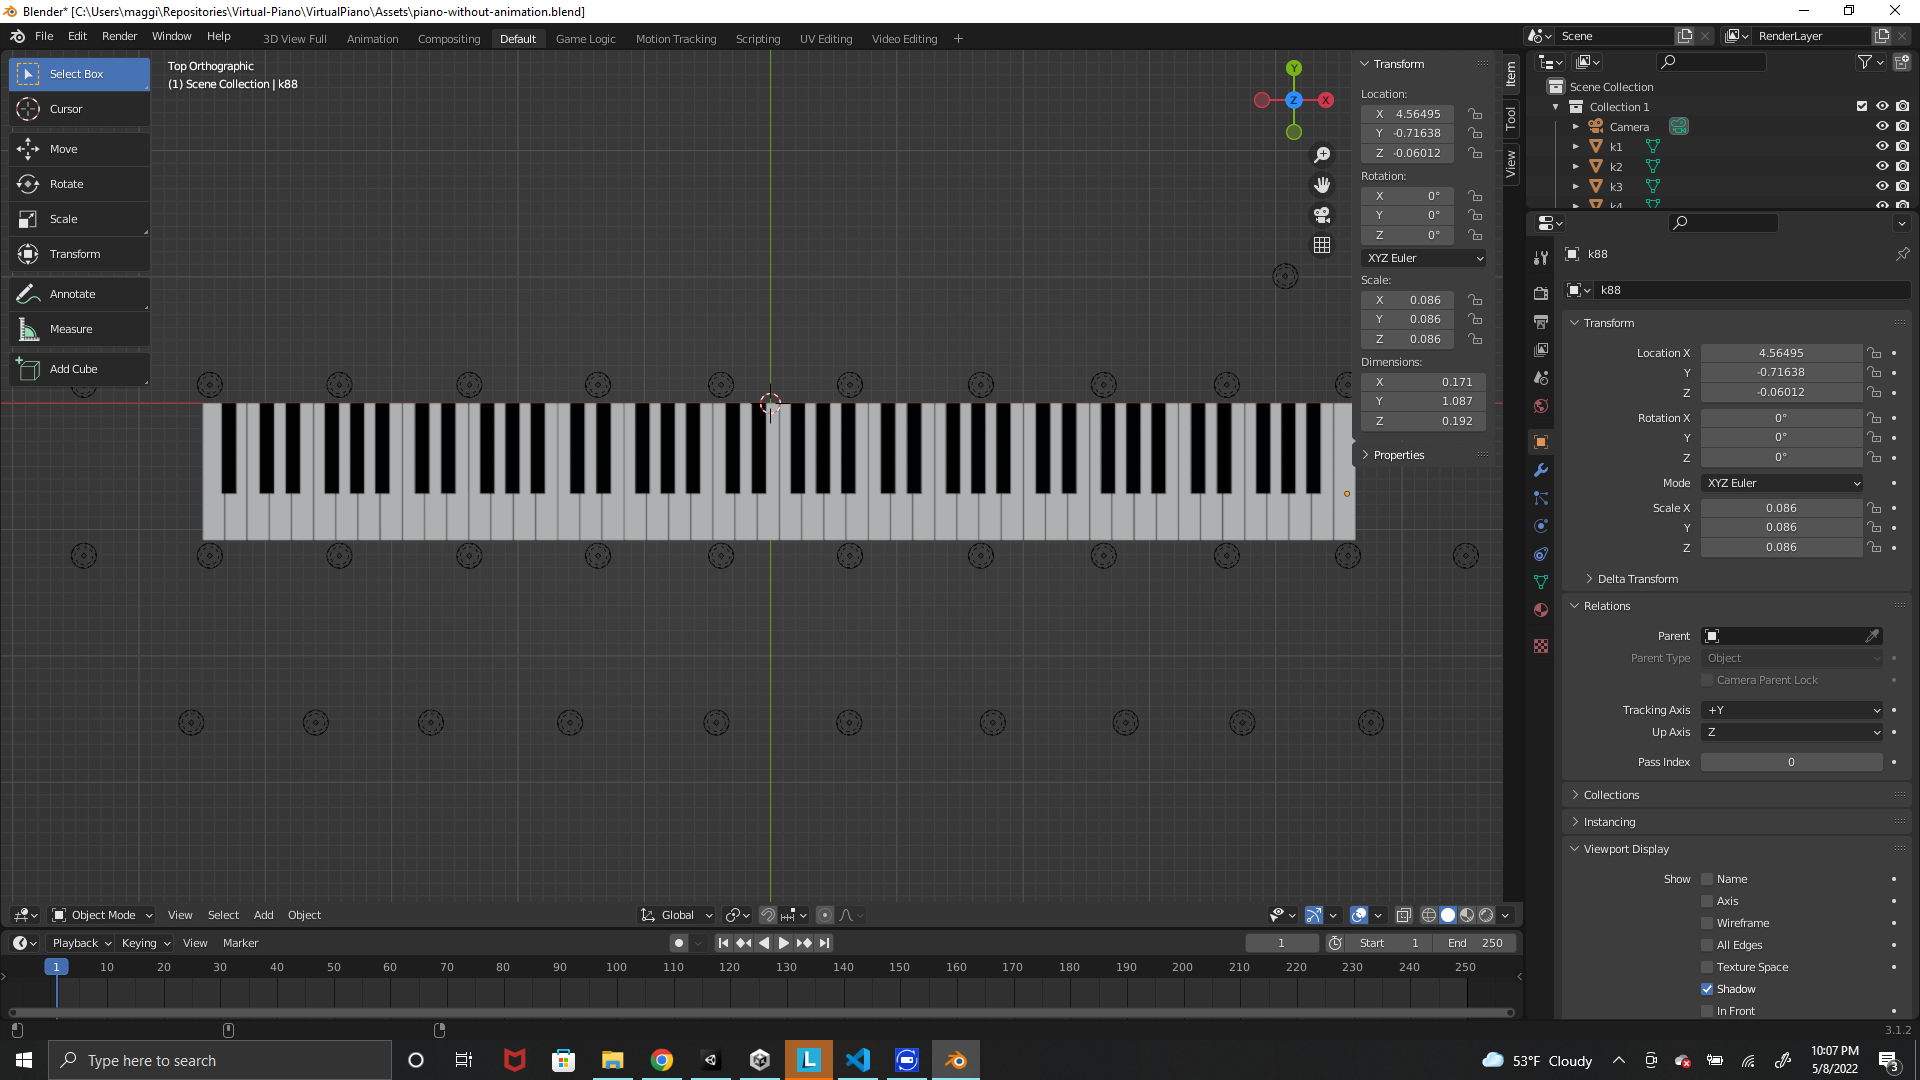
\includegraphics[width=8cm, height=5cm]{OriginalPiano.png}
\centering
\caption{The piano taken from the original project.}
\end{figure}

The intent of this study is to determine whether or not a virtual piano is a suitable replacement for a physical one in K-12 schools.  Because the end goal is to use this piano for educational purposes, I decided to take the original piano object, and color code each octave on the keys.  

\subsection{Procedure}
This experiment is set up as a within-subjects study involving a multi-part Qualtrics survey, where participants will be prompted to answer various questions and be asked to play a physical piano and a virtual piano.  

\subsubsection{Consent Form}
The first part of this survey is the consent form.  If someone does not consent to participating in the study, then the survey ends there.  Otherwise, they will continue through the survey questions and instructions.
\subsubsection{Demographics}
After the consent form, users will be asked to answer the following questions regarding their demographic information.  
\begin{enumerate}
 \item Gender (M/F/Other)
 \item Age
 \item Name (first and last)
 \end{enumerate}
\subsubsection{Playing the Real Piano}
After answering the demographic questions, users will be prompted to answer a few questions to gauge their previous experience with playing piano and other musical instruments.  The questions being asked are:
\begin{enumerate}
 \item Do you have experience playing the piano? (Not just hitting/playing random keys)
 \begin{enumerate}
 \item How long have you been playing the piano?
 \item What age did you start playing piano?
 \end{enumerate}
 \item Do you have experience playing any other instruments?
 \begin{enumerate}
 \item What instrument?
 \item How long have you been playing this instrument?
 \item What age did you start playing this instrument?
 \end{enumerate}
\end{enumerate}

Once they answer these questions, they will be instructed to play the physical piano.  Once they are done playing the physical piano, they can click the next button to move onto the virtual piano section of the survey.
\subsubsection{Playing the Virtual Piano}
While the virtual piano is an 88 key piano, you can only view a small section at a time, specifically 2 octaves.  Because of this, the participants were prompted to choose which two octaves they would like to play.  The options are:
\begin{enumerate}
 \item Octaves 1 and 2
 \item Octaves 2 and 3
 \item Octaves 3 and 4
 \item Octaves 4 and 5
 \item Octaves 5 and 6
 \item Octaves 6 and 7
 \end{enumerate}

After answering this question, I will set up the participant's chosen octaves.  The survey will then prompt the user to play the virtual piano.  Once they are done playing the virtual piano, they will click the next button to move onto the follow up section of the survey.

\begin{figure}[h]
\centering
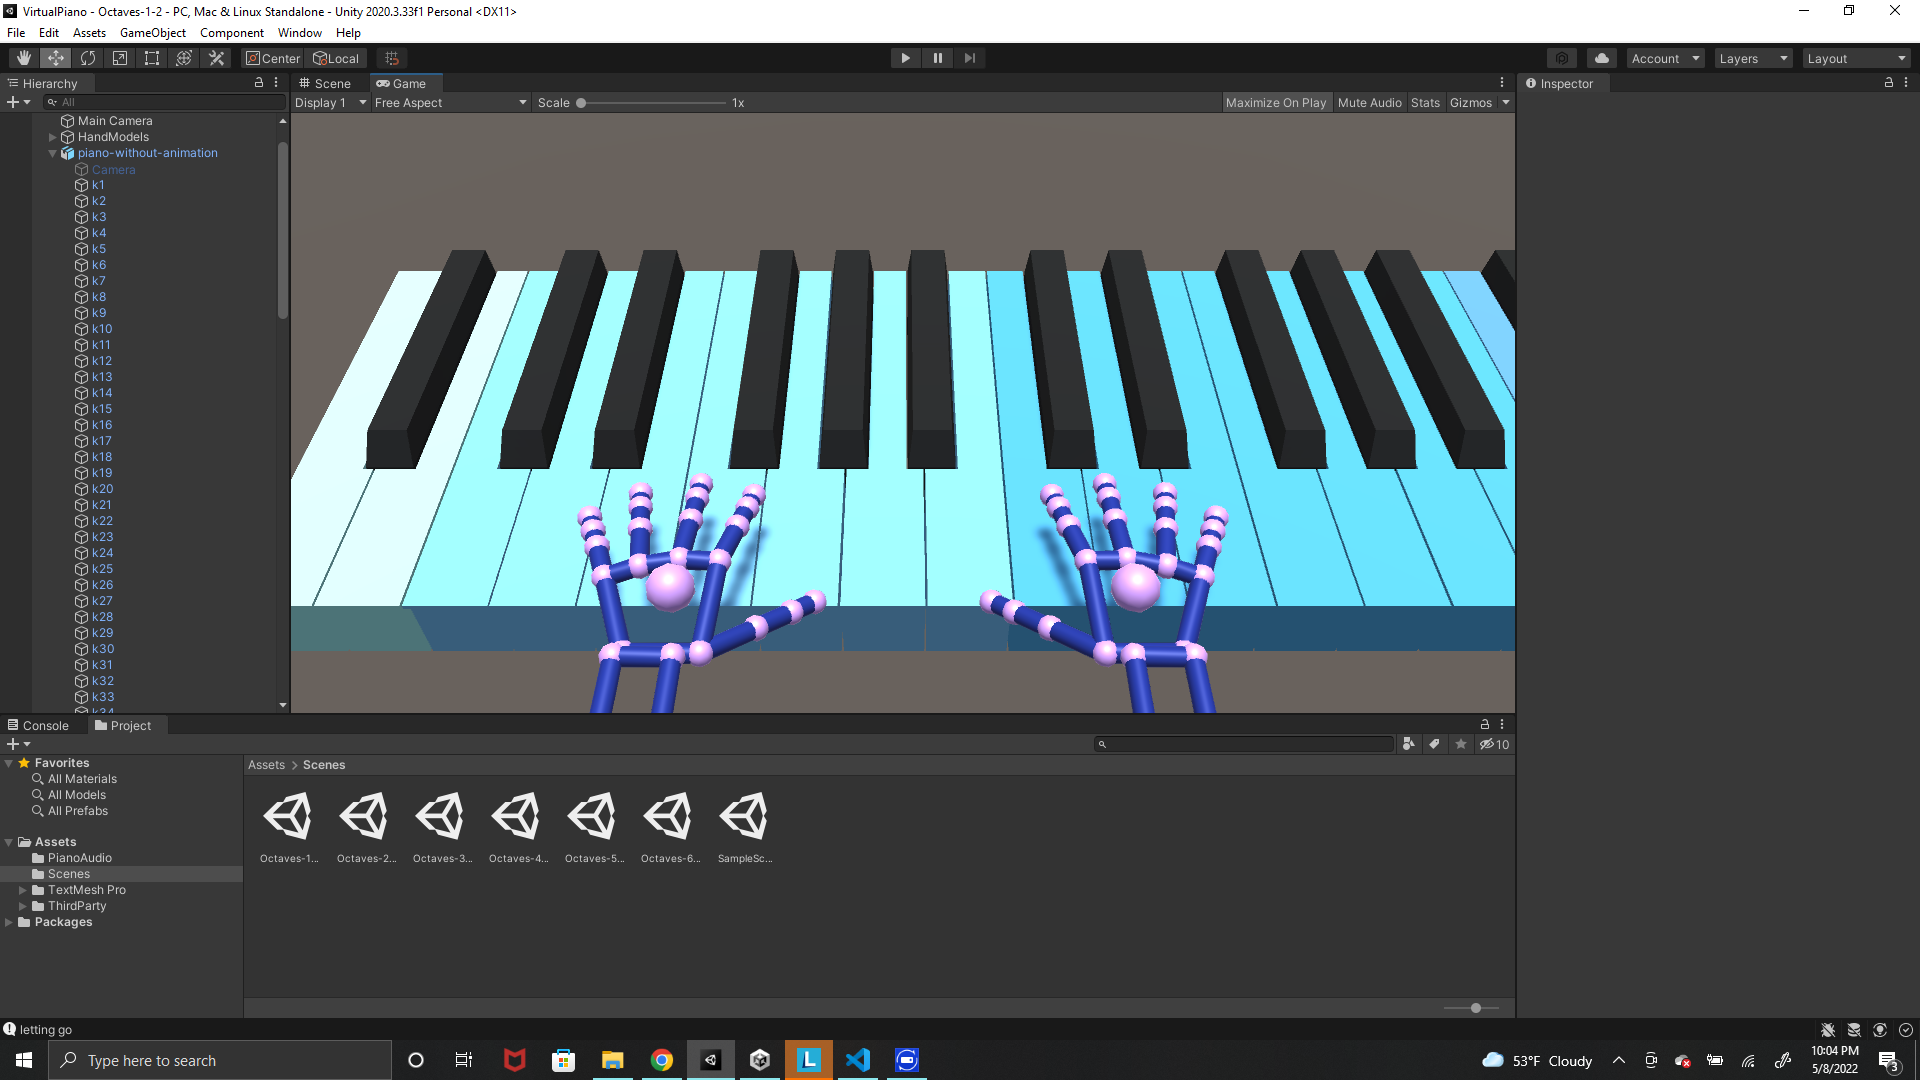
\includegraphics[width=8cm, height=5cm]{Octave1.png}
\centering
\caption{The first octave in the piano experiment}
\end{figure}

\subsubsection{Follow Up Survey}
The first part involves a questionnaire to collect demographics.  Each participant will be asked the following questions.
\begin{enumerate}
 \item Did you find the virtual piano easier or more difficult to play than the physical piano?
 \item Please rank the difficulty level of playing the physical piano and virtual piano on scale of 1 to 10 (1 = easy, 10 = hard).
 \item Did you attempt to play an actual song on the virtual piano?
 \begin{enumerate}
 \item Were you successful at playing said song on the virtual piano?
 \end{enumerate}
 \item With improvements and technological advancements, in the future, do you think virtual pianos could be a suitable replacement for a real piano?
 \item Do you think this specific virtual piano would be a suitable replacement for a real piano in K - 12 schools?
 \item Please write any feedback, if any, about the virtual piano (criticisms, ideas for improvement, etc.)
\end{enumerate}

\subsection{Design}
This study is set up to look at playing a real piano versus a virtual one, and has participants play both.  Because of that, the independent variable would be the instrument being played (the real one or the virtual one).  One of the dependent variables is the all the data collected from the survey regarding the differences between the real piano and the virtual one.  Another dependent variable is the octave the participants chose to play.  The control variable in this experiment is the instructions since every participant was given the same set of instructions.  Finally, the confounding variables is any previous experience participants have playing the real piano.

\section{Results/Analysis}
The results of the qualtrics survey gave good insights into whether or not participants have played the piano or any other instruments in the past.  Of the 10 participants, 3 played the piano growing up, all starting between the ages of 8 and 10, and continuing to play for 1 to 3 years.

\begin{figure}[h]
\centering
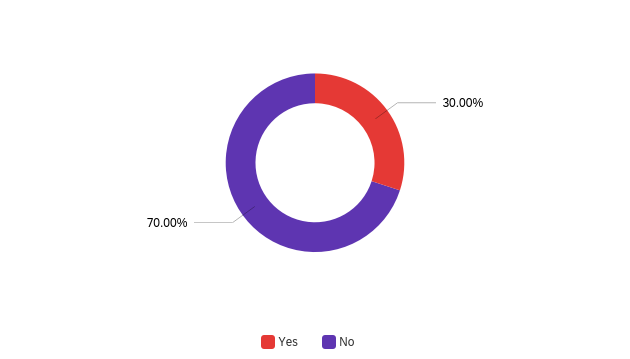
\includegraphics[width=8cm, height=5cm]{PianoExperience.png}
\centering
\caption{Participants' experience playing the piano}
\end{figure}

7 out of the 10 participants had played another instrument.  Of the 7 participants that played another instrument, 3 of them played guitar.  The other four participants played either the viola, the ukulele, the saxophone, or the flute.  They all started playing between the ages of 10 and 15, and played anywhere between 1 and 10 years.  Some of these participants played more than one instrument growing up, but they were instructed to put just one in the survey.

\begin{figure}[h]
\centering
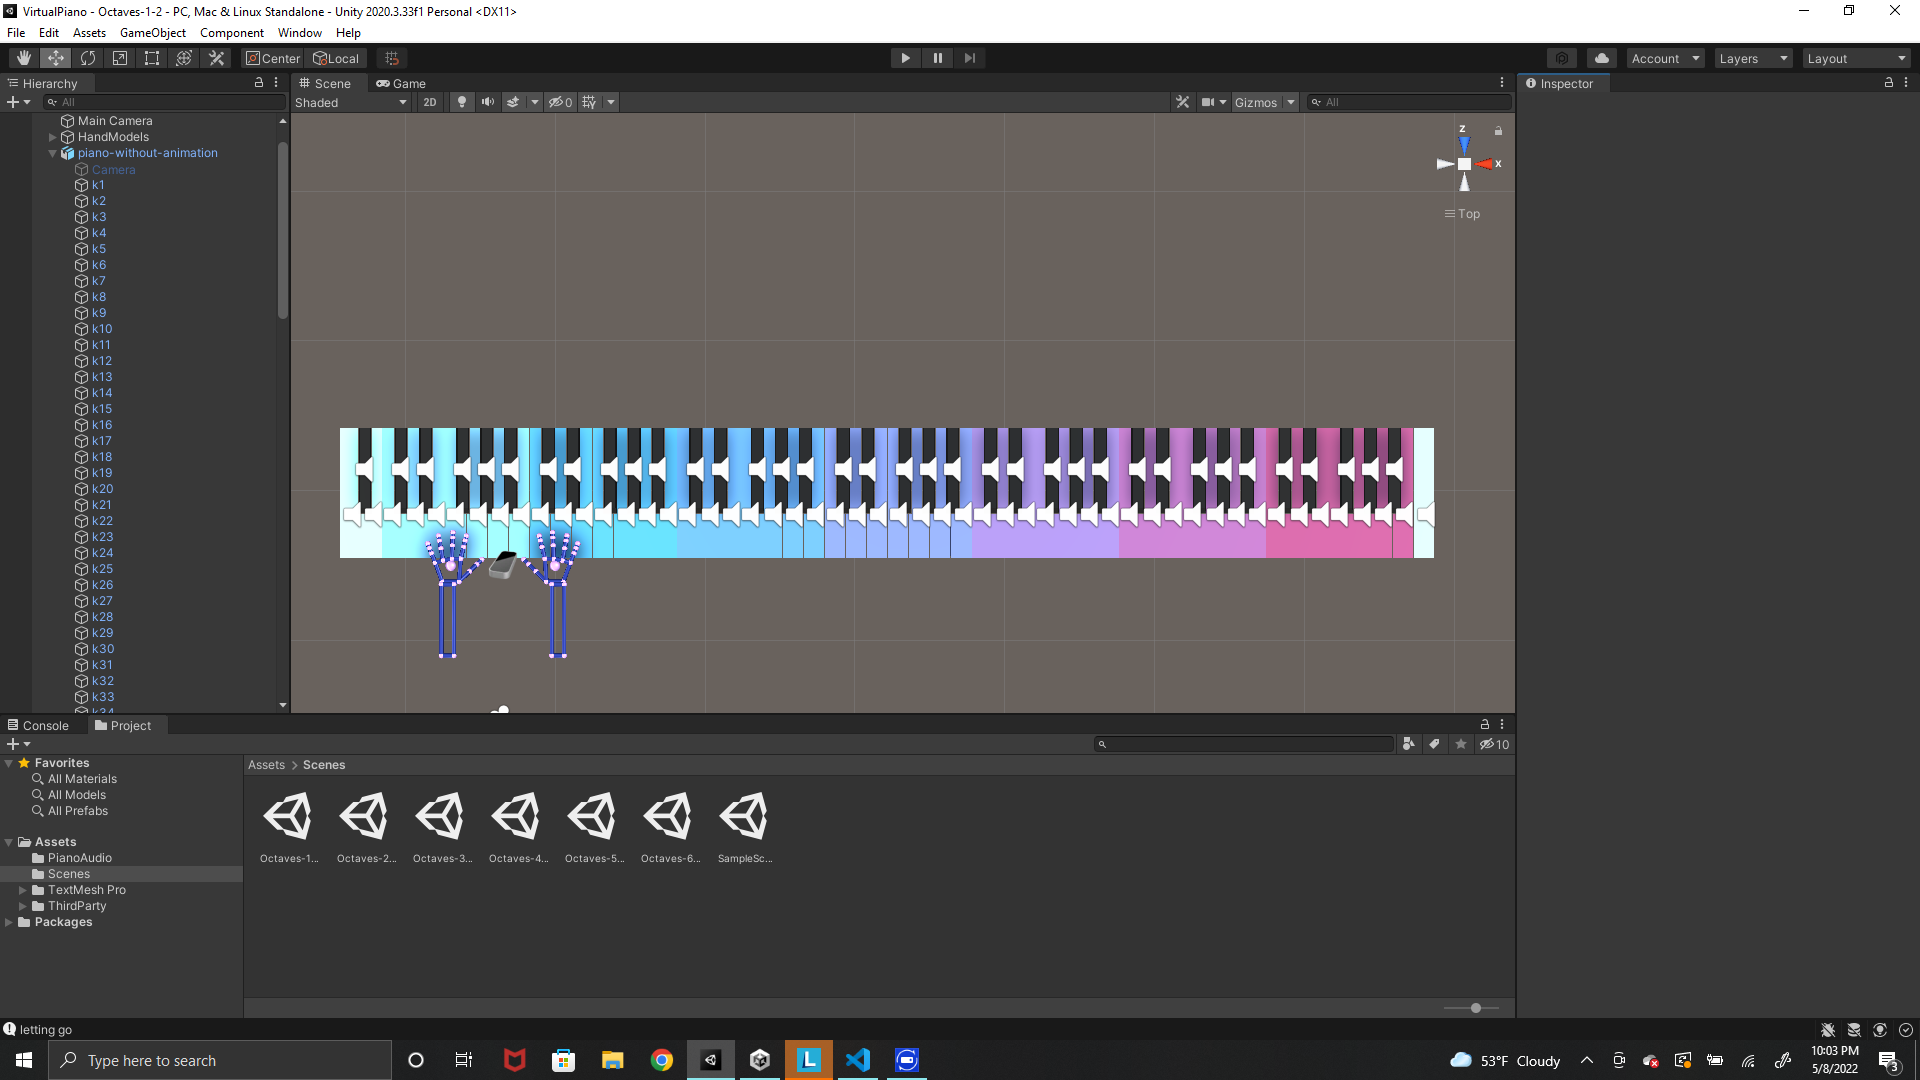
\includegraphics[width=8cm, height=5cm]{WholePiano.png}
\centering
\caption{The entire virtual piano, color coded by octaves.}
\end{figure}

Because the entire piano could not be played due to hand scaling issues with the leap motion device, participants had to choose which octaves they wanted to play.  Nearly all participants chose to play the third and fourth octaves.  Each of them were asked why, and they all said the same thing.  They felt like it was a good octave because it is in the middle of the piano.  Only one participant chose to play the first octave.

\begin{figure}[h]
\centering
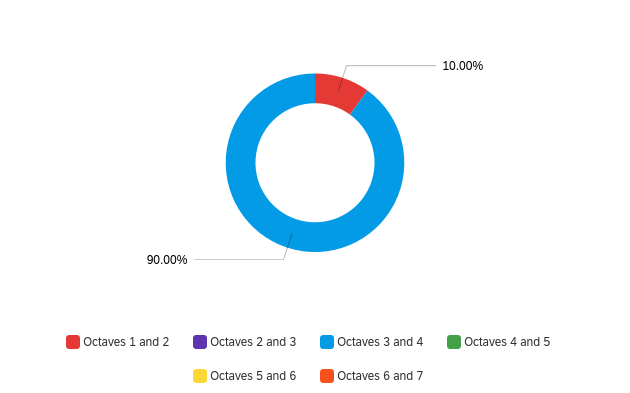
\includegraphics[width=8cm, height=5cm]{OctavesChosenBreakdown.png}
\centering
\caption{Octaves chosen by Participants}
\end{figure}


All participants said they found the virtual piano harder to play than the physical piano.  9 out of the 10 participants felt that with technological advancements, the virtual piano could be a suitable replacement for the physical piano.  When asked if they thought this specific piano could be a replacement for a physical one in K-12 schools, 6 participants said yes while 4 said no.

\begin{figure}[h]
\centering
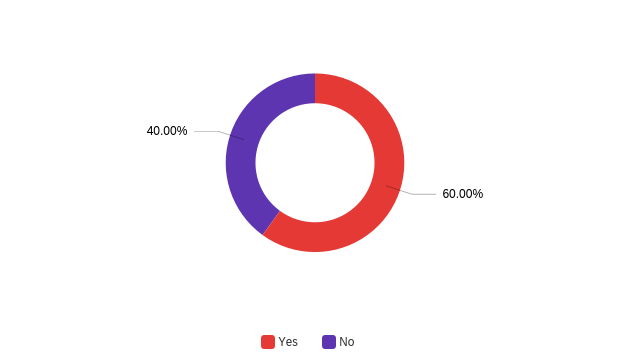
\includegraphics[width=8cm, height=5cm]{K-12 Question.png}
\centering
\caption{Responses from participants' when asked if the piano could be used in K-12 schools}
\end{figure}

Participants were also asked to provide any feedback they had regarding the piano functionality.  Many of them all had similar things to say about the sensor and the precision when hitting the piano keys.  One of the biggest complaints participant's stated while playing the piano was how difficult it was to hit the black keys.

\section{Conclusion}
Participants were almost split down the middle regarding if the current piano could be used in schools.  Because everyone had pretty similar complaints regarding the sensitivity and intended interaction, it seems that there would need to be some improvements made before it could be used in schools and be useful to students.

The placement of the sensor needs to have some more trial and error testing in order to determine the best position.  This is because it is hard to place it in a way so that it works perfectly every time.  One thing that came up with the participants, and in the building phases was how difficult it was to hit the left piano keys.  Placing the sensor so it was aligned in the center of the screen was not the best place as seems to not sense on both sides equally.  One thing that seemed to somewhat fix this issue was moving the sensor more towards the left so it was slightly off center.
%%
%% The acknowledgments section is defined using the "acks" environment
%% (and NOT an unnumbered section).  This ensures the proper
%% identification of the section in the article metadata, and the
%% consistent spelling of the heading.
% \begin{acks}
% To Robert, for the bagels and explaining CMYK and color spaces.
% \end{acks}

%%
%% The next two lines define the bibliography style to be used, and
%% the bibliography file.
\bibliographystyle{ACM-Reference-Format}
\bibliography{references}

%%
%% If your work has an appendix, this is the place to put it.
\appendix


\end{document}
\endinput
%%
%% End of file `sample-authordraft.tex'.
